% !Mode:: "TeX:UTF-8"
\chapter{视频编码原理与关键技术}
\label{cha:c2}
本章由简要的视频编码技术发展史开始,引出视频编码中最为核心的 5 项技术:预测编码、变换量化 (Transform and Quantization, TransQuant)、环路后处理、熵编码以及率-失真优化 (Rate-Distortion Optimization, RDO),为后文分析视频编码的可优化方向以及分析所提出算法的可行性打下基础。
在早期视频编码标准中并未包含上述所有核心技术,但随着各类应用对视频编码效率的需求日渐严苛,该 5 项核心技术被证明对编码效率提高起着核心作用,成为了缺一不可的存在。目前仍在征集提案的 H.266 标准的发展趋势亦是在该框架下再进行部分精细优化。

在正文之前,首先申明以下用词:
1) 统一使用视频“编码”而非视频“压缩”。在视频编解码领域,“编码”与“压缩”表达相同的含义,都指经过预测、变换量化、熵编码等操作达到减小数据冗余、压缩视频数据量的目的。编码是手段,压缩是目的,按照习惯统一使用视频编码这一表述,类似地,使用编码标准、编码方案、编码效率等表述;
2) 为了直接体现出编码标准的发展历程,不使用高级视频编码 (Advanced Video Coding, AVC)、高性能视频编码 (High Efficiency Video Coding, HEVC) 和多功能视频编码 (Versatile Video Coding, VVC) 的表述,统一使用 H.264、H.265 和 H.266,两类表述在含义上并无差异;
3) 由联合专家组维护的各标准参考模型随着版本迭代可能存在不同的命名,例如 H.266 的参考模型在早期曾称为 JEM(Joint Exploration Model),本文中统一使用以下命名:用于 H.264 的 JM(Joint Test Model) 模型\upcite{AVCsoftwareJM}、用于 H.265 的 HM(HEVC Test Model) 模型\upcite{HEVCsoftwareHM16}以及用于 H.266 的 VTM(VVC Test Model) 模型\upcite{VVCsoftwareVTM}。

\section{视频编码技术发展历史}
应用广泛的 H.265 与正在征集提案的 H.266 视频编码标准,是数字视频编码技术 40 年的研究和 30 年的标准化的成果,代表着各时期最先进的视频编码技术。在视频编码技术发展的早期(H.264 制定以前),国际上存在 2 套应用广泛的标准,分别是国际电信联盟-电信标准化部门 (International Telecommunication Union-Telecommunication Standardization Sector, ITU-T) 制定的 H.26X 系列,与国际标准化组织 (International Organization for Standardization, ISO) / 国际电工委员会 (International Electrotechnical Commission, IEC) 制定的 MPEG 系列。前者广泛应用于网络视频通信,后者主要应用于视频存储和广播流媒体。
H.264 以后的编码标准则是由 ITU-T 派出的视频编码专家组 (Video Coding Experts Group, VCEG) 和 ISO/IEC 派出的动态图像专家组 (Moving Pictures Experts Group, MPEG) 共同征集提案制定的。联合专家组在 H.264 时期称为联合视频组 (Joint Video Team, JVT);在 H.265 时期称为视频编码联合合作组 (Joint Collaboration Team on Video Coding, JVT-VC);在 H.266 早期称为联合视频探索组 (Joint Video Exploration Team, JVET),现在称为联合专家组 (Joint Video Experts Team, JVET)。

H.26X 标准自问世至今在整体框架上并未变动,如图 \ref{fig:BlockDiagram} 所示,包含帧内/帧间预测、变换量化、熵编码、环路后处理以及率-失真优化模块。但各代标准在上述 5 大模块中均加入了新的编码工具,使编码效率呈现出每代提高约 50\% 的趋势\upcite{H266Overview}。例如帧内预测模式自 H.264 的 9 种发展到了 H.266 的 67 种;变换量化过程经过拆分重组减小了计算复杂度;环路后处理方面 H.265 中引入了新的自适应补偿机制,大幅提高了图像质量。
\begin{figure}[hbt]
    \centering
    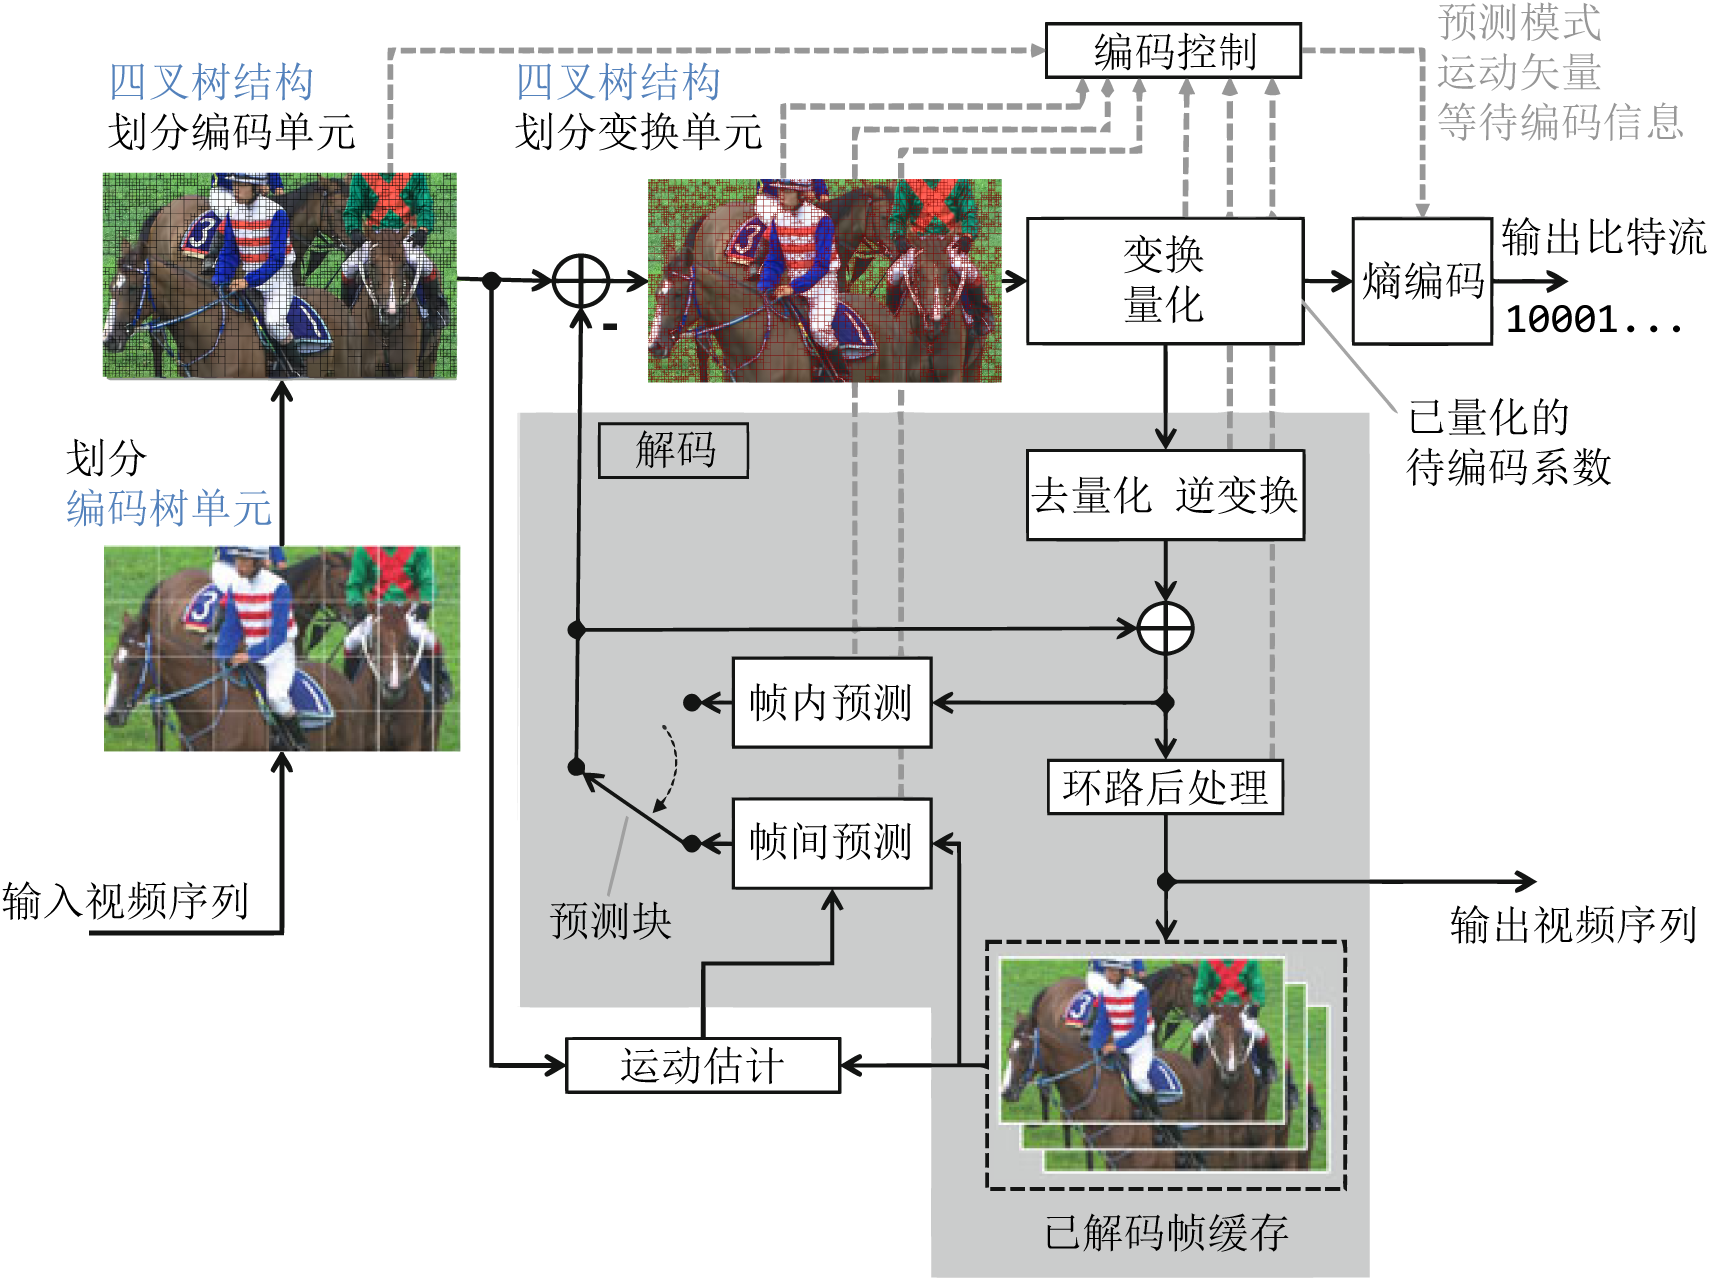
\includegraphics{BlockDiagram.png}
    \caption{H.26X 标准视频编码框架}
    \label{fig:BlockDiagram}
\end{figure}

\section{预测编码技术}
预测编码是 H.26X 系列编码标准中的重要组成部分之一。视频信号表现出很强的空间相关性和时间相关性,即在空间上相邻像素点之间的亮度或色差值相近,在时间上同一区域相邻两帧之间的像素点亮度或色差值相近。使用帧内和帧间预测技术可以准确地对像素值进行预测,进而编码预测值与原始像素值的残差,极大地减少视频信号的时空冗余。预测编码的基本流程如图 \ref{fig:PredicitonOverview} 所示。对于待预测像素 $x(n)$,首先利用已重建的像素结合特定的预测模式得到预测值 $p(n)$,然后计算预测残差 $e(n)$,最后对 $e(n)$ 进行变换、量化、熵编码,同时使用去量化、逆变换后的重建值 $e^{'}(n)$ 与预测值 $p(n)$ 重建出后续待预测像素的参考值 $x^{'}(n)$。
\begin{figure}[hbt]
    \centering
    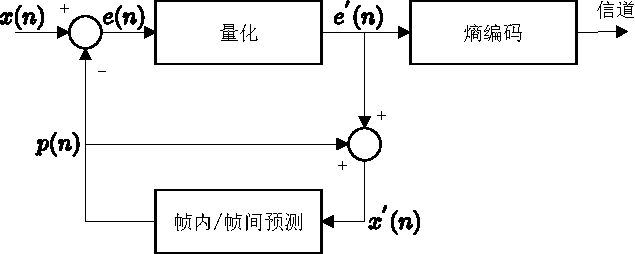
\includegraphics{PredicitonOverview.pdf}
    \caption{H.26X 预测编码的基本流程}
    \label{fig:PredicitonOverview}
\end{figure}

根据参考像素种类的不同,可将预测编码分为以下两类,在后文将进一步介绍:
\begin{enumerate}
    \item 帧内预测,即利用待预测点空间上临近的已重建像素点进行预测的方法;
    \item 帧间预测,即利用待预测点时间上临近的几帧(可以是之前也可以是之后)在相同位置附近的已重建像素点进行预测的方法。
\end{enumerate}

\subsection{帧内预测}
帧内预测指利用视频、图像的空间相关性,使用已编码重建的像素点预测当前像素,预测完成后的像素经过重建又作为后续待预测像素的参考点。设待预测点为 $f(x,y)$,$(x,y)$ 为待预测点坐标,该点的预测值由已重建的参考点 $\widetilde{f}(k,l)$ 进行预测给出:
\begin{equation}
    \widehat{f}(x,y) = \sum_{(k,l)\in Z}a_{k,l}\widetilde{f}(k,l)
\end{equation}
其中 $a_{k,l}$ 表示特定预测方式,多表现为投影与插值的组合,$Z$ 为参考点所在区域。后续变换量化、熵编码的对象均为预测值与原始值的误差,即预测残差 $e(x,y)$:
\begin{equation}
    e(x,y) = f(x,y) - \widehat{f}(x,y)
\end{equation}

H.26X 系列标准中制定了多种帧内预测模式,包括平滑预测(DC 模式、Planar 模式)和方向预测两大类。随着编码标准的发展,预测模式的数量不断增多,H.264 仅使用 9 种模式\upcite{H264Overview},H.265 增加到 35 种\upcite{H265Overview},H.266 达到了 67 种\upcite{H266Overview},显然模式越多越有可能得到精确的预测值,最后体现为更高的编码效率。
标准中,任意一种预测模式都是以相邻块的边界上的重建像素为参考点进行的,该方案使得每个预测单元 (Prediction Unit, PU) 均能自适应地选择最佳的预测模式。如图 \ref{fig:ModeFit} 所示,左侧衣物上存在明显的方向性条纹,适合使用方向预测模式,而右侧的衣物呈现出平坦的特性,适合使用 DC 或 Planar 模式。关于帧内预测的更详细的分析将在 \ref{cha:IntraPredDetail} 节进行。
\begin{figure}[hbt]
    \centering
    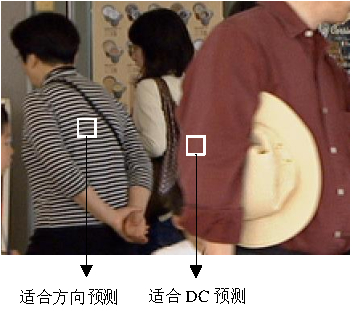
\includegraphics{ModeFit.pdf}
    \caption{选择不同的帧内预测模式}
    \label{fig:ModeFit}
\end{figure}

\subsection{帧间预测}
帧间预测指利用视频的时间相关性,使用临近帧(可以是之前也可以是之后)相同位置附近的像素点预测当前像素。以像素点为单位进行帧间预测显然是不可行的,因此与帧内预测类似,帧间预测也以块为单位,如图 \ref{fig:InterPredOverview} 所示。其预测策略是针对每个待预测块,从已编码的其他帧中寻找与其匹配的块作为参考块,计算参考块到待预测块的位移信息。该过程即为运动估计,其中得到的位移信息称为运动矢量,预测块与参考块的差值称为运动预测残差。
\begin{figure}[hbt]
    \centering
    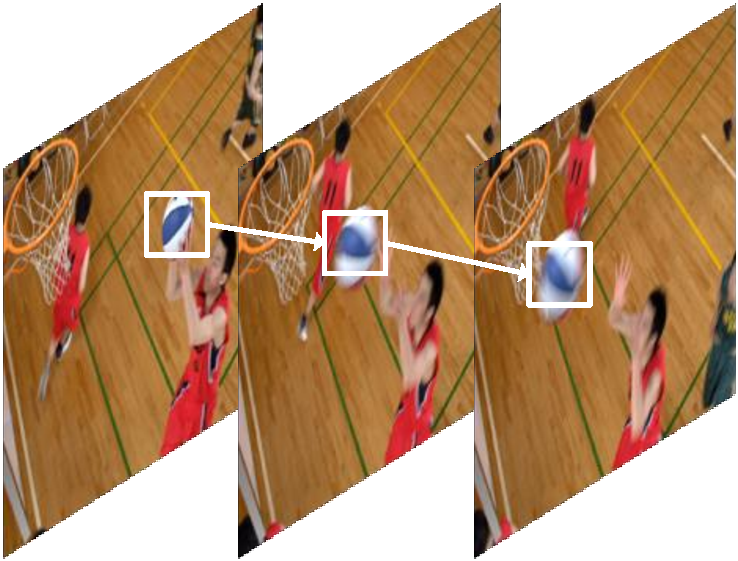
\includegraphics[scale=0.7]{InterPredOverview.pdf}
    \caption{H.26X 帧间预测}
    \label{fig:InterPredOverview}
\end{figure}

帧间预测中的核心技术是运动搜索算法,运动搜索是 H.26X 编码中最耗时但也是影响编码效率最大的一个过程。H.26X 标准中并未指定搜索方法而只在软件模型中给出了参考算法,例如 HM 模型中给出了全搜索算法和 TZSearch 算法\upcite{ImprovementsTZSearch}。全搜索算法指对于每一个待预测块,遍历搜索窗口中所有可能的运动矢量取其中运动预测残差最小的一个;TZSearch 算法属于快速算法的一种,其按照固定的菱形搜索模板或正方形搜索模板以 2 的整数次幂递增步长进行运动搜索,大幅减少搜索量的同时保持了较好的搜索性能(不容易陷入局部最优)。

\section{变换与量化技术}
H.26X 编码标准中,通过帧内和帧间预测获得了相对原始像素值能量大幅降低的预测残差,且预测编码并未引入失真。后续的变换与量化进一步地对残差进行处理,使能量集中得到稀疏的待编码数据,同时也是编码过程中真正引入失真的步骤。

\subsection{变换编码}
\label{cha:TransformOverview}
变换编码技术指将预测残差(某些特殊情况下是原始像素值)从空间域通过离散余弦变换 (Discrete Cosine Transform, DCT) 或离散正弦变换 (Discrete Sine Transform, DST) 转换到频域,以变换域系数来表示数据。本节以 DCT 为例简单介绍 H.26X 标准中变换编码的应用场景及效果。

DCT 是一种在频域对数字信号进行分析的工具,在数学上共有 8 种形式\upcite{FastFourierTransform},图像、音视频领域中常用的是 II 类 DCT:
\begin{equation}
    \begin{gathered}
        X(k) = \sqrt{\frac{2}{N}}\varepsilon_{k}\sum_{n=0}^{N-1}x(n)\cos\left[\frac{k(2n+1)\pi}{2N}\right], \quad k=0,1...,N-1 \\
        \varepsilon_{k}= \left\{
        \begin{aligned}
            \frac{1}{\sqrt{2}}, \quad & k=0 \\
            1, \quad                  & o.w
        \end{aligned} \right.
    \end{gathered}
    \label{equ:1ddct}
\end{equation}
当 $k=0$ 时式中不再有余弦项,即 $X(0)\propto$ 信号 $x(n)$ 的均值,此时称 $X(0)$ 为信号 $x(n)$ 的直流 (Direct Current, DC) 分量;反之,当 $k>0$ 时,$k$ 越大式中的余弦信号频率越高,此时 $X(k)$ 反映了信号 $x(n)$ 在不同频率分量上的分布多寡,称为信号 $x(n)$ 的交流 (Alternate Current, AC) 分量。

以 H.265 标准测试序列“BasketballPass”中第一帧的前 8 个数据 $x(n)$ 为例计算其对应的变换域系数 $X(k)$:
\[
    x(n): 127,129,130,128,125,122,123,124
\]
当 $k=0$ 时:
\[
    X(0)=\frac{1}{2\sqrt{2}}(127+129+130+128+125+122+123+124)\cos(0)\approx 356
\]
同理根据式 \ref{equ:1ddct} 计算所有的 $X(k)$ 得到:
\[
    X(k): 356,6,-1,-4,0,0,0,0
\]
从上述示例中可以看出,当原始信号 $x(n)$ 的数值分布比较均匀即各数值之间相关性强时,其变换域的系数 $X(k)$ 将呈现出数值集中分布在 DC 和低频部分的稀疏状态。显然,自然图像中的像素幅值或其预测残差都很容易表现出强相关性,因此将待编码数据转换到变换域十分有利于后续的熵编码。另外,上述示例是 II 类 DCT 的一维形式,实际上图像、视频编码中使用的是其二维形式:
\begin{equation}
    \begin{gathered}
        X(k,l)=C(k)C(l)\sum_{m=0}^{N-1}\sum_{n=0}^{N-1}x(m,n)\cos\left[\frac{(2m+1)k\pi}{2N}\right]\cos\left[\frac{(2n+1)l\pi}{2N}\right], \\
        % k,l=0,1...,N-1
        C(k)=C(l)=
        \begin{cases}
            \sqrt{\frac{1}{N}}, \quad k,l=0 \\
            \sqrt{\frac{2}{N}}, \quad 1 \leqslant k,l \leqslant N-1
        \end{cases}
    \end{gathered}
    \label{equ:2ddct}
\end{equation}

变换编码技术在 H.26X 中存在较多研究和优化内容不再赘述,但以下几点值得一提:
\begin{enumerate}
    \item DCT 去相关性的性能随着变换大小的增大而增强,但增强的比率迅速减缓,因此考虑到计算复杂度和编码性能的折衷,较常采用的是 4x4 与 8x8 DCT,很少用到 16x16 及更大的变换;
    \item 同样出于计算复杂度的考虑,从 H.264 开始标准中的变换一般拆分为两部分进行,即与浮点运算无关的整数变换部分及分离出的比例缩放系数\upcite{IntergerDCTs},后者将与量化合并为一次计算,提高了计算效率;
    \item 根据统计结果,对 4x4 大小的亮度块预测残差使用 DST 能提高约 0.8\% 的编码效率而计算复杂度不变\upcite{DCTDSTchoose},因此从 H.265 开始将 DST 纳入考虑;
    \item 哈达玛变换与 DCT 处理后的变换残差绝对值之和 (Sum of Absolute Transformed Difference, SATD) 相近,但哈达玛变换计算复杂度极低,因此 H.265 将哈达玛变换与 SATD 作为快速预测模式选取的工具。
\end{enumerate}

\subsection{量化}
从 H.264 将变换拆分为整数变换和比例缩放两部分以后,H.26X 标准中产生失真的原因集中到了量化上(图 \ref{fig:TransQuantCombine})。H.26X 标准中仅规定了量化过程的解码方法,将编码端量化方式的选择策略交给编码器自行设计和优化,H.265 中可选的量化方法有传统标量量化、自适应量化 (Adaptive Quantization) 和率-失真优化量化 (Rate-Distortion Optimization Quantization, RDOQ),本节以标量量化为例介绍量化的过程和作用。
\begin{figure}[hbt]
    \centering
    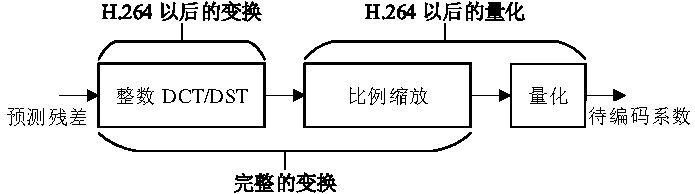
\includegraphics{TransQuantCombine.pdf}
    \caption{H.26X 中变换量化过程的拆分与合并}
    \label{fig:TransQuantCombine}
\end{figure}

由于经过变换后的数据动态范围很大,需要通过量化将数据的取值范围压缩才能得到理想的编码效率。经过压缩必定会产生数据精度损失,因此量化是音视频编码中产生失真的根本原因,也是控制编码结果码率的最直接因素。标量量化的过程如下式:
\begin{equation}
    l_i=\left\lfloor \frac{c_i}{Q_{step}}+f \right\rfloor
\end{equation}
其中 $c_i$ 表示 \ref{cha:TransformOverview} 节所述的变换域系数,$Q_{step}$ 为量化步长,$l_i$ 为量化器的输出,$f$ 用于控制舍入。
H.265 中可选 52 个量化步长,量化步长小代表数据精度损失小即失真小但同时编码效率低。
需要注意量化并非简单地对输入的变换域系数平等地做缩放。基于人类视觉系统 (Human Visual System, HVS) 研究中发现的人眼对亮度、低频分量敏感,对色差、高频分量较不敏感的生物特性,各类图像视频编码方案中均存在量化矩阵的概念。即对不同频率分量的变换域系数做相应的缩放,例如对低频分量做更轻微的量化以保证良好的视觉效果。
值得一提的是相对于学术界关注峰值信噪比 (Peak Signal-to-Noise Ratio, PSNR)、结构相似度 (Structural Similarity Index, SSIM)\upcite{PSNRSSIM} 等客观图像质量评价指标,工业界更关心的是平均主观得分 (Mean Opinion Score, MOS),即实验者根据自身的观看体验给出的图像视频质量分数,工业界中甚至有关于“让人感觉舒服,错以为图像质量好的失真”的研究,此为另外的研究方向不再展开。
总之量化是控制视频质量的关键步骤,量化系数的选择策略尤为重要。

\section{环路后处理技术}
H.26X 标准中的预测、变换和量化等编码工具均是基于块结构设计的,相邻块之间由于预测模式突变、量化值突变和不属于同一个变换单元 (Transform Unit, TU) 等多方面原因,产生了不可避免的数值不连续性。人眼对此类不连续性较敏感,导致视频编码后的 MOS 大打折扣。对此 H.26X 对重构像素进行后处理作为应对,因该处理处于预测-变换-量化-重建环路中而称为环路后处理(图 \ref{fig:BlockDiagram}),包含去方块滤波 (Deblocking Filter) 和 H.265 中新增的像素自适应补偿 (Sample Adaptive Offset, SAO)。
\subsection{去方块滤波}
去方块滤波技术从 H.264 开始引入,其作用是消除相邻编码块间的不连续性,一方面可以直接优化视频的视觉效果提高 MOS,另一方面经过去方块滤波的数据更适合作为后续编码单元 (Coding Unit, CU) 的参考点,使预测值更加精准,间接提高了 PSNR 和 SSIM 等客观指标。需要注意的是并非所有的编码块边缘都需要进行去方块滤波,图像中纹理信息丰富的编码块之间必然存在较强的不连续性,此时进行去方块滤波不仅无法提升视觉质量还会导致图像中的细节丢失。因此去方块滤波的基本原则是对数值平滑的编码块之间存在的不连续性做强滤波,对本身数值波动较大的编码块之间存在的不连续性不做滤波或只做弱滤波,如图 \ref{fig:TypicalDB} (a) (b) 所示。因此,去方块滤波在具体实现中分为了滤波决策与执行滤波两个步骤,执行滤波也分为亮度分量强滤波、亮度分量弱滤波和色差分量滤波 3 类,具体不再展开。
\begin{figure}[hbt]
    \centering
    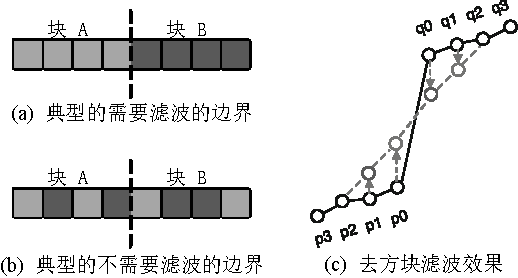
\includegraphics{TypicalDB.pdf}
    \caption{去方块滤波应用场景及效果}
    \label{fig:TypicalDB}
\end{figure}

\subsection{样点自适应补偿}
SAO 是 H.265 新引入的环路后处理技术。H.26X 标准中为了得到稀疏的待编码系数进行了量化,量化的对象是变换域系数,而量化不可避免地会产生数据失真,变换域系数的数据失真通过逆变换回到空间域则表现为重建值在原始值的附近上下波动,如图 \ref{fig:Gibbs} 所示。
\begin{figure}[hbt]
    \centering
    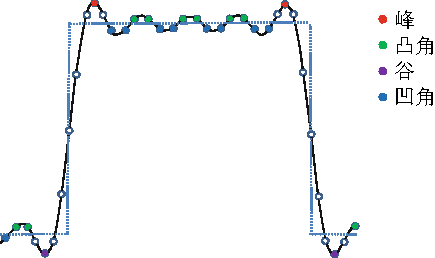
\includegraphics{Gibbs.pdf}
    \caption{量化失真引起的振铃效应}
    \label{fig:Gibbs}
\end{figure}

这种波动在数学上称为吉布斯现象,在图像视频编码领域更形象地称为振铃效应。振铃效应的成因是变换域的高频分量系数产生的失真过大,因此“振铃”在图像细节丰富的区域尤为明显。为了减轻振铃效应带来的图像质量损失,H.265 标准应用了一种十分直接的处理方案:对重建数据进行后处理,在“振铃”的“谷”添加正补偿,在“振铃”的“峰”添加负补偿。在具体的补偿方案中又分为边界补偿 (Edge Offset, EO) 和边带补偿 (Band Offset, BO),本节仅以 EO 为例介绍 SAO 的处理过程。

边界补偿采用对每个像素点单独进行分类和补偿的策略,出于性能与复杂度的折衷,分类过程仅涉及待处理像素及其相邻的 2 个像素。H.265 中需要通过 SAO 进行补偿的像素点共有 4 类,如图 \ref{fig:SAOCategories} 所示。
\begin{figure}[hbt]
    \centering
    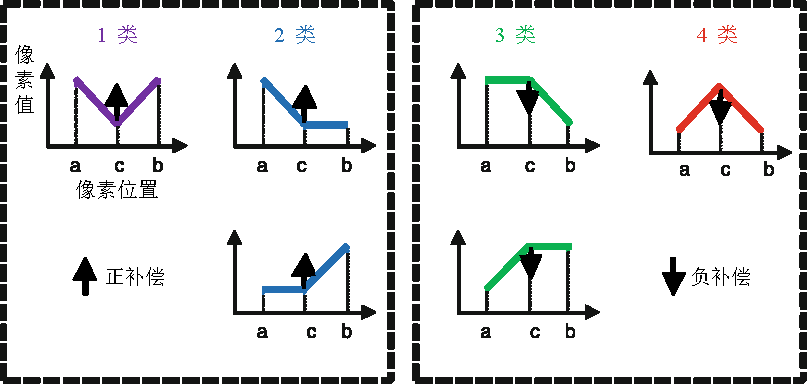
\includegraphics{SAOCategories.pdf}
    \caption{SAO 边界补偿分类}
    \label{fig:SAOCategories}
\end{figure}

对于 1 类“谷”和 2 类“凹角”进行正补偿,将使补偿点附近更加平滑;对于 3 类“凸角”和 4 类“峰”进行负补偿,同样使补偿点附近平滑。对于不属于上述 4 类的像素点将归类为 0 类不进行补偿。在预先定义了补偿的正负性后,编码器仅须记录绝对补偿值,解码器便可通过同样的分类策略进行补偿。因此 SAO 在保证了仅传输极少量数据的情况下对图像视频质量做出了有效的优化。

\section{熵编码技术}
熵编码是 H.26X 标准中编码的最后一步,其将各类待编码的数据转换为具有特定语法语义的二进制比特流(见图 \ref{fig:BlockDiagram})。因其依据信息熵理论进行优化而称熵编码,熵编码可进一步利用待编码数据的统计特性消除冗余,是提高视频编码效率的重要工具。

\subsection{变长编码在视频编码中的应用}
对不同的输入符号使用不同长度的码字进行编码称为变长编码。为了得到更高的编码效率,需要将短码字分配给出现频率高的符号,反之将长码字分配给几乎不出现的符号以使平均码字长度最短。值得一提的是,变长编码中各码字必须符合“任意一个码字的尾缀不能是其他任意码字的前缀”的要求,否则变长码将不可译(在不添加码字间分隔符的情况下),符合该要求的一组码字一定是“唯一可译码”。

经典的哈夫曼码是一种最佳变长码,然而在解哈夫曼码时解码器必须依靠编码端提供的哈夫曼树结构,因此增加了编码、传输的数据量,另外解哈夫曼码时需要一次性读入大量码流在树中搜索匹配码字,复杂度过高。因此早期的图像编码中使用了固定结构的范式哈夫曼编码,如 JPEG。另一类方案是使用有固定规则的编码方法,如 H.26X 中使用的指数哥伦布码 (Exponential Golomb Code)。指数哥伦布码的构建过程如下,其中 $k$ 表示阶数:
\begin{enumerate}
    \item 将待编码数值表示为 2 进制,分离出尾部 $k$ 位,剩余部分加 1;
    \item 计算剩余部分有几位,减去 1 后得到的结果为码字前缀 0 的个数;
    \item 将 1 中分离出的尾部 $k$ 位重新补回。
\end{enumerate}
表 \ref{tab:ExpColombCode} 给出了 0 阶和 1 阶的部分指数哥伦布码字,较小的数值被分配到了更短的码字。在 H.265 中指数哥伦布码多用于各类参数信息的编码,如视频参数集 (Video Parameter Set, VPS)和序列参数集 (Sequence Parameter Set, SPS) 等均使用 0 阶指数哥伦布码进行编码。
\begin{table}[hbtp]
    \centering
    \caption{$k$ 阶指数哥伦布码}
    \label{tab:ExpColombCode}
    \begin{tabular}{@{}crr@{}}
        \toprule
        \textbf{阶数}          & \textbf{码字}                     & \textbf{编码范围} \\ \midrule
        \multirow{5}{*}{$k$=0} & 1                                 & 0                 \\
                               & 0 1 $x_0$                         & 1...2             \\
                               & 0 0 1 $x_1$ $x_0$                 & 3...6             \\
                               & 0 0 0 1 $x_2$ $x_1$ $x_0$         & 7...14            \\
                               & ...                               & ...               \\
        \multirow{5}{*}{$k$=1} & 1 $x_0$                           & 0...1             \\
                               & 0 1 $x_1$ $x_0$                   & 2...5             \\
                               & 0 0 1 $x_2$ $x_1$ $x_0$           & 6...13            \\
                               & 0 0 0 1 $x_3$ $x_2$ $x_1$   $x_0$ & 14...29           \\
                               & ...                               & ...               \\ \bottomrule
    \end{tabular}
\end{table}

\subsection{算术编码在视频编码中的应用}
尽管变长编码提高了编码效率,但对于每个输入符号使用变长编码至少都要 1 比特表示。算术编码解除了这种限制,其本质是对整个输入序列分配 1 个码字,平均来看可能实现用少于 1 比特的数据量来表示一个符号。算术编码的过程简述如下:
\begin{enumerate}
    \item 统计输入序列中所有符号出现的概率;
    \item 根据编码符号对应的概率将区间 $[0,1)$ 进行分配,区间的大小正比于概率,某符号分配到区间 $[L, H)$;
    \item 从初始区间 $[0,1)$ 开始,设置:
          \begin{equation}
              low=0, \quad high=1 \nonumber
          \end{equation}
    \item 按顺序读入待编码符号,根据其分配到的 $[L, H)$ 对区间进行更新:
          \begin{equation}
              \begin{aligned}
                  low  & =low+(high-low)*L \\
                  high & =low+(high-low)*H
              \end{aligned} \nonumber
          \end{equation}
    \item 最后得到区间 $[low, high)$,选择下界 $low$ 作为该序列的算术编码码字。
\end{enumerate}

在上述过程开始前确定了各符号的概率进行编码的称为静态算术编码,显然这在视频编码中是无法实现的。因此 H.26X 在进行算数编码的过程中对信源符号的概率不断建模、更新,该技术发展到 H.265 成为了成熟的基于上下文的自适应二进制算术编码 (Context-Based Adaptive Binary Arithmetic Coding, CABAC)。其核心是编码过程中维护了一个设计精良的上下文模型,每个符号的编码均与以前的编码结果有关,根据输入待编码符号流的统计特性自适应地分配码字。H.265 中与待编码系数有关的大量语法元素采用的都是 CABAC,如变换跳过标志、编码块标志以及帧内/帧间标志等。

\subsection{模式依赖的编码顺序}
量化后的待编码系数普遍具有幅值小且稀疏的特性,有效地利用这一特性可以使 CABAC 的上下文建模更加高效。H.26X 标准中的编码工具均是基于块设计的,因此在最后一步的熵编码之前,如何将二维分布的待编码数据按特定的顺序扫描送入熵编码器在标准中也进行了规定。扫描的顺序需要进一步考虑数值的空间分布特征,将幅值相近的数据集中在一起扫描有利于上下文建模,从而提高编码效率。

H.265 中规定扫描的过程分为 4x4 子块间的扫描与 4x4 子块内的扫描,块间与块内扫描递归进行。具体的扫描顺序又分为水平扫描、垂直扫描和对角扫描,制定该 3 类扫描顺序的根据是预测模式与系数分布特征间的联系:一个采用(接近)垂直预测模式得到的待编码块,其能量很可能集中在前几行,因此水平扫描对(接近)垂直预测模式的块有利,同理垂直扫描对水平预测模式的块有利,对此 \ref{cha:IntraPredDetail} 节将做进一步分析。图 \ref{fig:ScanOrder} 给出了具体的 3 类扫描顺序。
\begin{figure}[hbt]
    \centering
    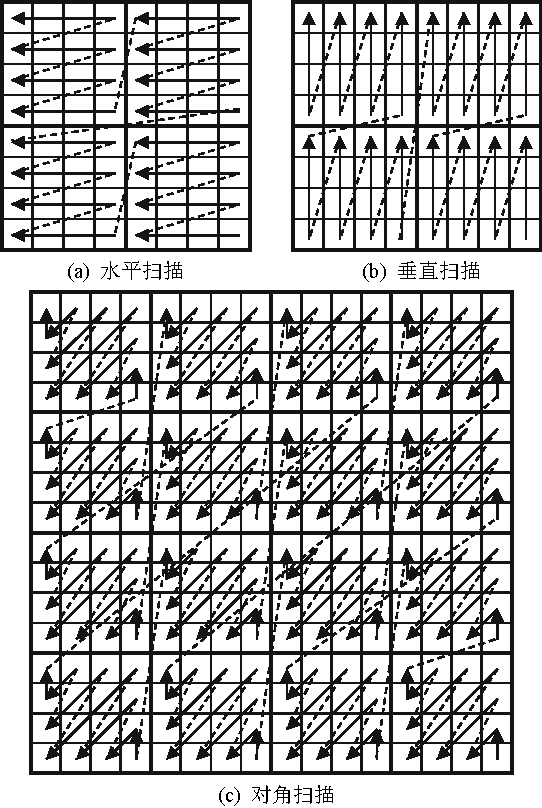
\includegraphics{ScanOrder.pdf}
    \caption{H.265 待编码系数扫描顺序}
    \label{fig:ScanOrder}
\end{figure}

与传统图像编码如 JPEG 不同,H.265 的扫描始终从最后一个系数开始到 DC 系数结束,与 Zig-Zag 扫描恰好相反。值得一提的是上述扫描的单位固定为 4x4 系数块,不论该块在预测、变换时是何种尺寸,这一限定有利于具体实现时的模块化操作。

\section{率-失真优化技术}
视频编码标准中的大部分内容是指定各类语法和语义,只要是符合标准语法语义的码流都能称为符合某视频编码标准。例如在使用 H.265 进行编码时,若将最小 PU 限定为 32x32(HM 默认配置是 4x4),编码效率与失真度可以预见甚至不如简单的 M-JPEG(Motion Joint Photographic Experts Group)。同时,为了适应不同的场景需求,视频编码标准中存在许多可配置参数用于调控编码效率、失真度和编码复杂度,因此,如何在标准的编码框架下得到最优的编码效率与失真度的平衡,是编码标准中未规定的算法研究的核心内容,寻找折衷点的过程被称为率-失真优化。

由于 H.26X 标准中未规定率-失真优化的具体技术细节,因此编码器可自定义、优化参数选择的过程。
率-失真优化方法可在图像组 (Group of Pictures, GOP) 层、片 (Slice) 层、编码树单元 (Coding Tree Unit, CTU) 层、CU 层和 PU 层应用。
\begin{itemize}
    \item GOP 的率-失真优化

          由于帧间预测的存在,各帧图像的编码效率和失真度存在相互依赖的关系,因此要得到最优的一组编码配置参数只能通过穷举的方法。GOP 层的穷举复杂度最高无法在实际编码中应用,因此 GOP 层的率-失真优化简化为独立确定各帧图像的最优编码配置参数。

    \item Slice 的率-失真优化

          Slice 是 H.265 中相对独立的编码单元,一个 Slice 包含多个相邻的 CTU,帧内/帧间预测时不能使用当前 Slice 外的参考像素。与 GOP 类似,当前 Slice 级别即各 CTU 之间的率-失真相关性还未被系统地考虑,仍按照独立确定各 CTU 的编码参数进行。

    \item CTU 的率-失真优化

          CTU 是 H.265 中基本的编码单元,CTU 一般会往下切分为多个 CU,CU 可切分为多个使用不同预测策略的 PU,PU 可选择适合自身的预测模式。由此 CTU 的率-失真优化分为 CU/PU 切分和 PU 的模式选择。类似地为了降低复杂度,当前 CU 的优化结束后不再考虑其对后续 CU 的影响。

    \item CU 的率-失真优化

          CU 层的优化任务是确定 PU 的预测模式和变换单元 (Transform Unit, TU) 的分割。目前 CU 级别的穷举复杂度可被接受,因此部分编码器在 CU 的优化过程中遍历候选集找出率-失真代价最小的一组参数。

    \item PU 的率-失真优化

          PU 层的优化任务是确定使用帧间预测还是帧内预测,以及具体的预测模式。以帧内为例,H.265 提供了 35 种可能的预测模式,可通过遍历的方法计算所有率-失真代价得到最优的预测模式。部分编码器如 HM 应用了哈达玛变换来加速这一过程(见 \ref{cha:TransformOverview} 节)。
\end{itemize}

\section{软、硬件视频编码开源项目}
互联网开源精神是当今学术界与工业界发展的重要推手,而视频编解码这一涉及到成像系统、生物信息、数学、统计学、计算机以及集成电路的庞大学科,如果没有一个系统的开源项目让各学科的研究人员参与进来,而是由单一的某一组织闭门造车是无法得到长足发展的。本小节总结了目前常用的软、硬件视频编码开源项目,本课题就是基于其中部分项目开展的。
\subsection{软件视频编码开源项目}
\begin{itemize}
    \item JM\upcite{AVCsoftwareJM}

          JM 是制定 H.264 标准的 JVT 负责维护的 H.264 编解码参考软件。JM 是学术界常用的编码器,其实现了 H.264 的所有特性,内部没有使用多线程或进行汇编层级的优化,因此其编解码速度较慢无法实现实时编码,多用于研究和测试标准性能。

    \item x264

          x264 是由 VideoLAN 维护的 H.264 编码器。x264 是工业界最常用的 H.264 编码器,其内部集成了丰富的快速、并行算法,使得编解码效率得到了极大提升,被应用在各类开源音视频处理框架中。目前最完善的多媒体处理软件 FFmpeg 在 H.264 部分就内嵌了 x264 用于编码。

    \item HM\upcite{HEVCsoftwareHM16}

          HM 是制定 H.265 标准的 JCT-VC 负责维护的 H.265 编解码参考软件。HM 是学术界在研究 H.265 和下一代视频编码标准时常用的编码器,其实现了 H.265 的所有特性(包括部分未写入标准的会议提案),内部没有使用多线程或进行汇编层级的优化,因此其编解码速度较慢无法实现实时编码,多用于研究和测试标准性能。

    \item VTM\upcite{VVCsoftwareVTM}

          VTM 是制定 H.266 标准的 JVET 负责维护的 H.266 编解码参考软件,随着 H.266 编码提案的征集仍在快速迭代中,在 H.266 标准探索的初期曾称为 JEM。VTM 是联合小组在制定下一代视频编码标准 H.266 时使用的编码器,用于测试所征集提案的性能。

    \item VVenC\upcite{VVCsoftwareVVenC}

          VVenC(Fraunhofer Versatile Video Encoder) 是在考虑到 VTM 过于庞大冗杂的编码工具后,根据多种复杂度优化提案在编码性能和编码时间之间取折衷的 H.266 编码器。维护者来自 VTM 开发的主要参与方、H.266 标准制定的重要参与者 Fraunhofer HHI。
\end{itemize}

\subsection{硬件视频编码开源项目}
\begin{itemize}
    \item OpenASIC Encoder RTL IP

          OpenASIC H.264/H.265 Encoder RTL IP 是由复旦大学微电子学院视频图像处理科研团队发布的 H.264/H.265 开源 RTL IP,由开源芯片社区 OpenASIC 共同维护。其中 H.264 Encoder RTL IP 实现了 H.264 标准编码流程,最大支持 1920x1088@30fps 实时编码,已被部分公司、研究所研究使用;H.265 Encoder RTL IP 发布了 2 个版本,实现了帧内/帧间预测、熵编码、环路后处理以及基础的码率控制,满足 0.13$\mu$m 工艺 400MHz 无时序违例综合,最大支持 4K@30fps 实时编码。
\end{itemize}

\section{本章小结}
本章简述了视频编码技术和标准的发展史,介绍了视频编码中的 5 项核心技术:帧内/帧间预测、变换量化、环路后处理、熵编码以及率-失真优化,为后文探索编码性能优化的可行性打下基础。